
\section{Differences between natural images and remote sensing surveys}\label{diffLidarNat}
Traditional work in object detection focusses on what we will call "natural images", which are photographs of scenes seen in normal settings. For examples, people sitting at a table, or children in front of horses. They are similar to images we would see with our own eyes. This means that, if there is an object in a photograph, there is a high probability that this object also exist and is the same category in the real scene that has been photographed. In other words, there is a good correspondence between the real object, its classification, and the kind of signal it emits in the visual field. A photograph of a camel will contain a camel, and we are able to very confidently classify the image as containing a camel, even though we are only classifying a \textit{visual representation}, not the object itself.

\begin{figure}[h]
	\begin{subfigure}[t]{.5\textwidth}
  \centering
  % include first image
  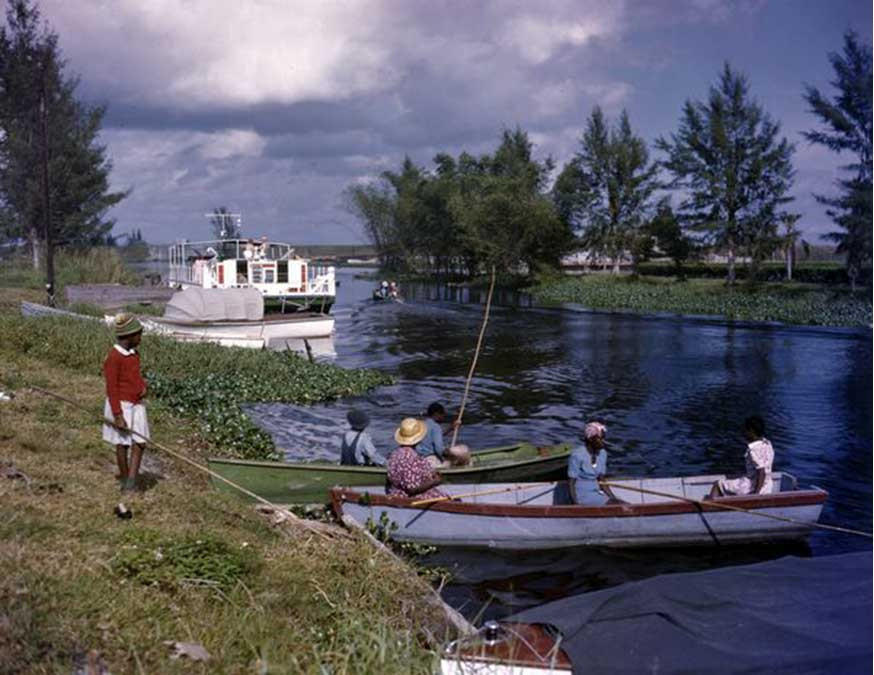
\includegraphics[width=\linewidth]{coco}  
	\caption{A natural image, taken from the COCO\cite{msCOCO} dataset}
  \label{fig:cocoEx}
\end{subfigure}
	\begin{subfigure}[t]{.5\textwidth}
  \centering
  % include second image
  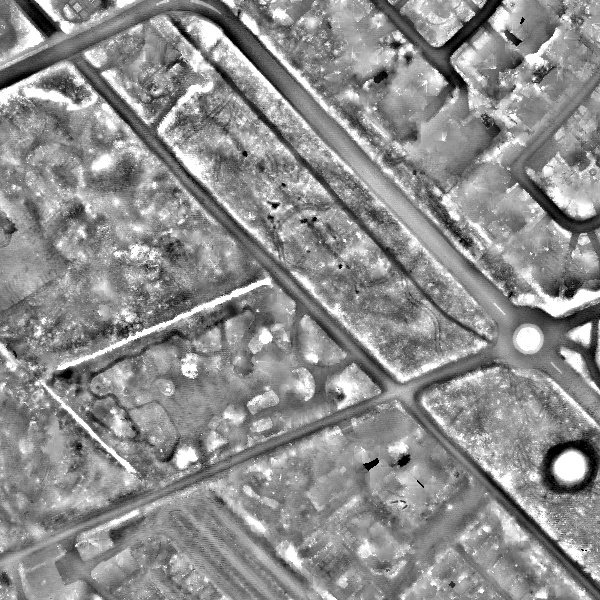
\includegraphics[width=\linewidth]{lidarEx}  
		\caption{An example from the \gls{lidar} dataset. On the bottom right, we can see an example of a barrow. However, this barrow is very similar to the roundabout seen slightly above.}
  \label{fig:lidarEx}
\end{subfigure}
	\caption{A natural image \textit{versus} a \gls{lidar} image}
\label{fig:cocovslidar}
\end{figure}

In remote sensing surveys, or more generally with any kind of image that is not made of purely visible light, the difference between the representation and the real object is more pronounced, and while it might be easy to detect and classify objects in the representation, to guarantee that those detected objects always match up with a real object is much more tricky. How can we say that the white mass seen in an X-Ray scanner that we detect and classify as a tumor is not only indeed a tumor in its representation, but also match up with a real tumor in a patient? The problem is even more prevalent with remote sensing surveys, with noise and geological details adding yet another layer of complexity.

\section{Occlusion and Vegetation}
Occlusion is a common issue in object detection, as more often than not object are not perfectly visible and are obscured by others. This issue is even more prevalent in detection of Archaeological structures. 

In the classes of objects that we aim to detect, most of them are quite sizeable and during construction of newer buildings or roads, those are often seen as obstacles to be removed, and part of them might be constructed upon. This hinders the visibility of those objects, and can pose a problem in detection.

Vegetation can also cause issues in the case of remote sensing surveys and wooded area can be prohibitively hard to analyze due to the occlusion created by trees\cite{kenzlerLambers2015}. With \gls{lidar} it can be possible to remove some of the occlusion caused by vegetation by carefully analyzing the return signal from the laser, but this might not be applicable with other type of remote sensing data.

\section{Issues with detection in remote sensing surveys}%TODO:Change title !
Whereas in natural images might be around a thousand pixels in width, remote sensing surveys cover hundreds of kilometer square of area, and are often tens of thousands of pixels wide. Moreover, the size of the object to detect is tiny in comparison to the size of the image, which is not usually the case in natural images. Traditional object detection techniques take advantage of this by heavily downscaling the image through the layers of the network, greatly reducing the computational cost. This is not possible to do with remote sensing surveys: a barrow, which might be a few meters wide in reality will be only a few pixels wide, and by downscaling we might lose all informations concerning those small objects. Those issues are similar with detection in satellite imagery, described in Van Etten\cite{yolt}, which might indicates that ideas used to mitigate them might also be applicable in our case.

When working with remote sensing surveys, one must always keep in mind those issues. In our case, the only reliable way of classifying archaeological objects is by prospecting and physical inspection, something that \textbf{cannot be done using only remote sensing surveys}. However, this create another issue, one of scale. The dataset comprised of 16 \gls{lidar} images. Each image has a very large resolution, $13140 \times 10290$, and cover about $30\text{km}^2$ of terrain. In its entirety, the dataset contains the position of about 3000 objects located around about $\sim 480\text{km}^2$ of terrain. It would be impossible for me to verify the correctness of every object in the dataset, because a definitive confirmation would imply a physical verification on site.

In short, even if the network architecture is fit for the task and trained properly, an already hard task, and even if the annotations in the dataset are entirely correct something that is even harder to do, we will still have an uncertainty as to whether the detected objects are not only actually real, but of the correct class. 

Tying this in with the ideas developed above: doing detections in remote sensing surveys, be it of Archaeological objects or otherwise, we should have some skepticism in the detections. Both because geophysical representations of objects are not always trustworthy, and because our detection system, as good as it can be, might always make mistakes.

\section{Dataset}\label{diffDataset}
In of itself, it is quite challenging to obtain large segments of \gls{lidar} surveys, or for that matter any kind of remote sensing surveys that is annotated. Deep Learning techniques usually requires vast amount of data to train properly. However, here  data can be prohibitively expensive to produce: a geophysical survey of an area is itself a challenge, with funding to secure and planning to be done. Moreover, annotating those dataset especially with Archaeological targets require experts and is very time consuming. Those two characteristics can render the annotation of such a dataset very complicated.\cite{kokaljHesse2017}

In Archaeology, the practice of Open Data, the act of freely sharing the data produced, is not yet widely adopted for a multitude of reasons. One of them is the possibility of looting. Since those surveys can show very clearly the presence of a potential archaeological object who might contain valuables such as gold, sharing this data to the world might make the act of looting easier\cite{optizHerr2018}.  

